\documentclass[11pt]{article}
\topmargin=0.0in %length of margin at the top of the page (1 inch added by default)
\oddsidemargin=0.0in %length of margin on sides for odd pages
\evensidemargin=0in %length of margin on sides for even pages
\textwidth=6.5in %How wide you want your text to be
\marginparwidth=0.5in
\headheight=0pt %1in margins at top and bottom (1 inch is added to this value by default)
\headsep=0pt %Increase to increase white space in between headers and the top of the page
\textheight=9.1in %How tall the text body is allowed to be on each page

\usepackage{url}
\usepackage{graphicx}
\usepackage{authblk}
\usepackage{wrapfig} % added from executive summary
\usepackage{etaremune}
\usepackage{hyperref}
\usepackage{amsthm}
\usepackage{amsmath}
\usepackage{listings} 
% \usepackage{draftwatermark}
% \SetWatermarkText{DRAFT}
% \SetWatermarkScale{5}
% "define" Scala
\lstdefinelanguage{scala}{morekeywords={class,object,trait,extends,with,new,if,while,for,def,val,var,this},
otherkeywords={->,=>},
sensitive=true,
morecomment=[l]{//},
morecomment=[s]{/*}{*/},
morestring=[b]"}
% Default settings for code listings
\lstset{frame=tb,language=scala,aboveskip=3mm,belowskip=3mm,showstringspaces=false,columns=flexible,basicstyle={\small\ttfamily}}

\renewcommand\Authfont{\fontsize{12}{14.4}\selectfont}
\renewcommand\Affilfont{\fontsize{9}{10.8}\selectfont}

\theoremstyle{plain}

\widowpenalty=500
\clubpenalty=500
\setlength{\parskip}{3pt}

\date{}

\begin{document}

\title{Annotating Regulatory Variants With \texttt{Fig}}
\author{Frank~Austin~Nothaft}
\maketitle

\begin{abstract}
Although large scale sequencing experiments such as the 1,000 Genomes Project have given
us a good understanding of the distribution of variants in the human population, many
questions about these variants still remain. Many questions surround the function of
variants seen in the non-coding regions of the genome. While the ``grammar'' used to
turn coding sequence into proteins is well understood, the effects of non-coding variants
can currently only be assessed through statistical measures such as GWAS and eQTL studies.

In this paper, we introduce \texttt{Fig}, a tool that \textbf{F}inds \textbf{I}nteresting
\textbf{G}enotypes by annotating non-coding variants. \texttt{Fig} uses a proposed grammar,
as well as known transcription factor binding sites to annotate haplotypes of variants.
We implement \texttt{Fig} using the \texttt{ADAM} API, and evaluate variant calls from the
third phase of the 1,000 Genomes project.
\end{abstract}

\section{Introduction}
\label{sec:introduction}

The recent $10,000\times$ drop in the cost of genome sequencing has enabled population
scale DNA and RNA sequencing experiments. Experiments such as the 1,000 Genome
Project~\cite{100012} and The Cancer Genome Atlas~\cite{cancer13} have allowed us to
analyze patterns of variation across large cohorts, which has led to an improved
understanding of both population-level variance, and the relationship between genetic
variation and diseases like cancer.

Although these experiments have provided us with a large set of data about human variation,
several large questions remain. One large question pertains to the role of variation
that occurs outside of the coding portions of the human genome. Although projects
such as ENCODE~\cite{gerstein12} have profiled the interaction of regulatory elements
with genomic sequence, these projects merely provide a glimpse into the interaction
between sequence and regulatory effects. While there is an emerging literature that
is studying the ``grammatical architecture'' of regulatory regions~\cite{levo14,
weingarten14}, this literature largely depends on synthetic experiments~\cite{sharon12}
to drive inference. While the results from these synthetic experiments are valuable, and
will improve our ability to model the impact of variants on regulation, we instead
seek to ask if there is a way for us to understand this relationship from existing
variation datasets?

In this work, we present \texttt{Fig}, a tool that applies ``grammar'' to annotate
the effect of variants called near regulatory sites. In the remainder of this paper,
we present summary results from looking at phase 3 of the 1,000 Genomes project,
and explain our methods. As this is preliminary work, we focus on the opportunities for
extending this work. Although we have not tackled this problem in this work, we believe
that this technique will prove useful for filtering out the importance of individual
variants that occur in linkage disequilibrium~(LD) blocks, which complicate studies that
look to statistically derive relationships between variation and expression~(expression
quantitative trait loci tests, eQTL) or phenotypes (genome wide association studies, GWAS).

\section{Results}
\label{sec:results}

We ran \texttt{Fig} on phased genotype data from phase 3 of the 1,000 Genomes project.
To annotate transcription factor binding sites~(TFBS), we used data from the ENCODE
project that was compiled by Kheradpour and Manolis~\cite{kheradpour14}. For reproducibility,
we have made the scripts used to run this experiment available from
\url{https://https://github.com/fnothaft/fig/blob/run-scripts/fig_analysis.sh}. We
annotated all regions that were 0 to 1,500 base pairs~(bp) ahead of the transcription
start site for all annotated genes\footnote{We used the GRCh37 gene annotations
available from \url{ftp://ftp.ensembl.org/pub/release-75/gtf/homo_sapiens/}.}.

First, we looked at the number of variants that occurred in the annotated regions.
This is depicted in Figure~\ref{fig:variants}. Interestingly enough, although most
annotated regions do contain a variant, approximately 43\% of annotated regions
do not contain variants. This is lower than expected, as the variation rate
in the human genome is 0.1\%\footnote{This rate actually underestimates the rate of
variation in a \emph{single} individual. Specifically, studies such as the 1,000
Genomes project have identified that approximately one ``common'' variant (present
in $>5$\% of the population) appears per 1,000bp.} Under a Binomial distribution with
$p = 0.001$ and $n = 1500$, we expect only 22\% of regions to not have variants.

\begin{figure}[h]
\begin{center}
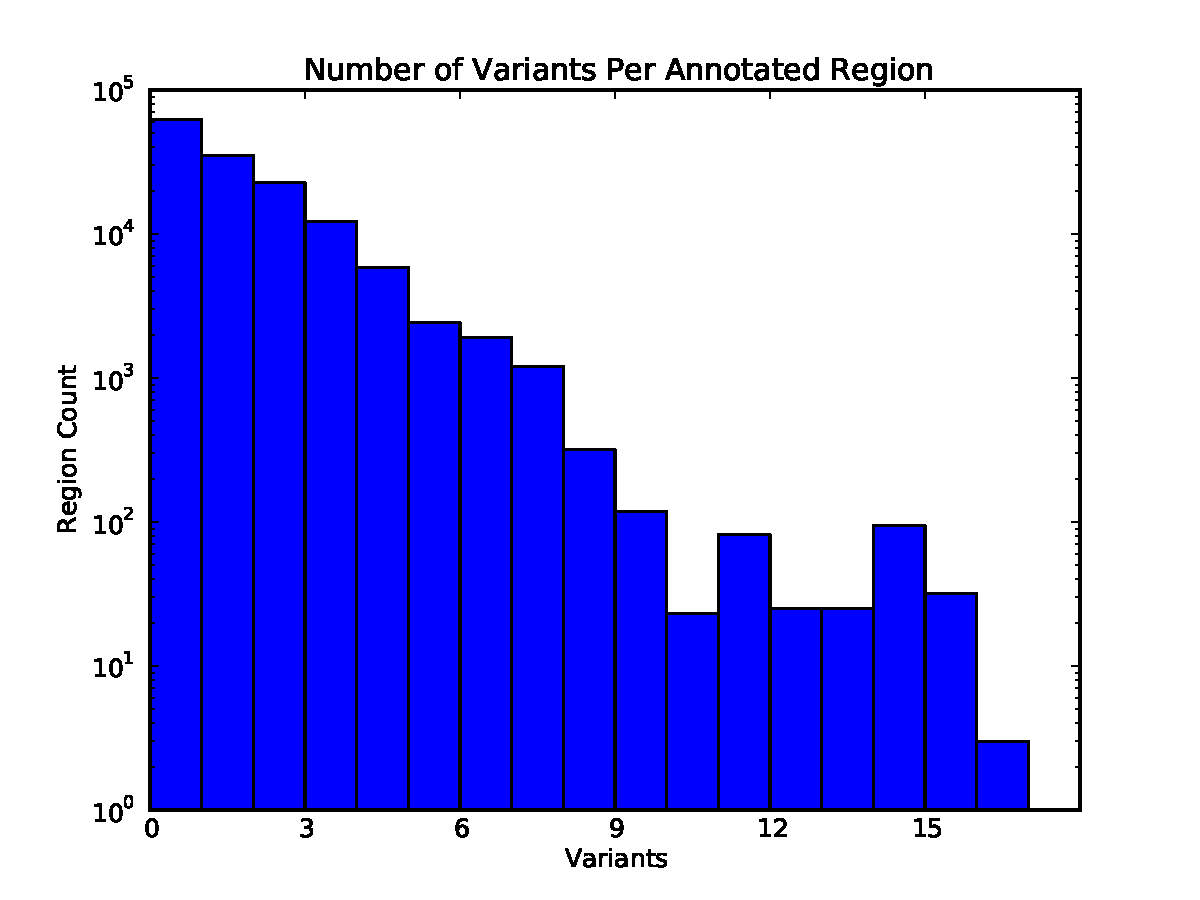
\includegraphics[width=0.25\linewidth]{graphs/variants.pdf}
\end{center}
\caption{Number of variants per region}
\label{fig:variants}
\end{figure}

After looking at this, we looked at the number of sites that were modified. This
data is shown in Figure~\ref{fig:sites}. We looked at the number of sites that
were lost, or the number of sites that were modified. We found that very few sites
were lost. The vast majority of regions did not lose a single TFBS, and the most
TFBS lost in a single region was 4. We would like to examine this closer to identify
the characteristics of regions that lost multiple sites. For example, this effect
could occur because of clustered variation (such as a multiple nucleotide polymorphism
or medium size INDEL), or because of a variant at a site that is overlapped by
multiple TFBS.

\begin{figure}[h]
\begin{center}
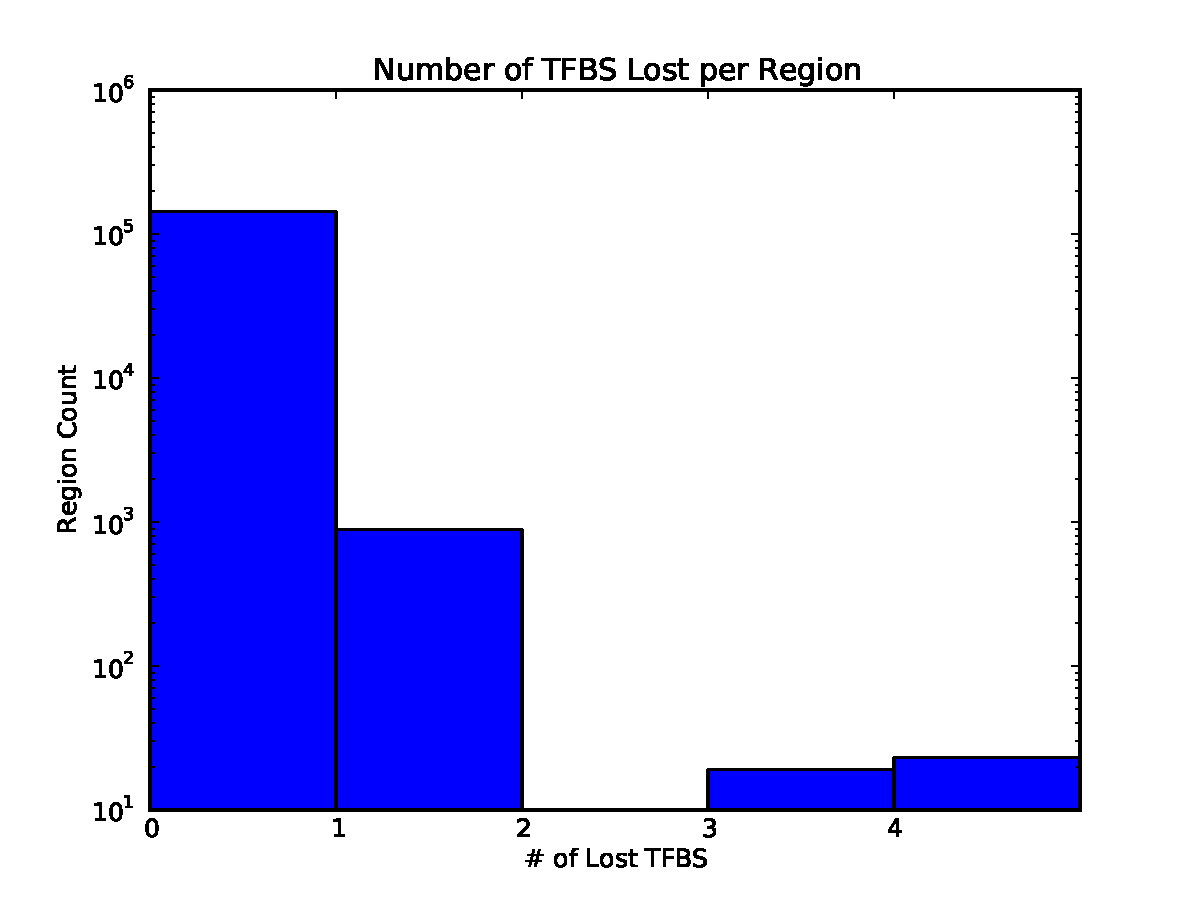
\includegraphics[width=0.25\linewidth]{graphs/lost-sites.pdf}
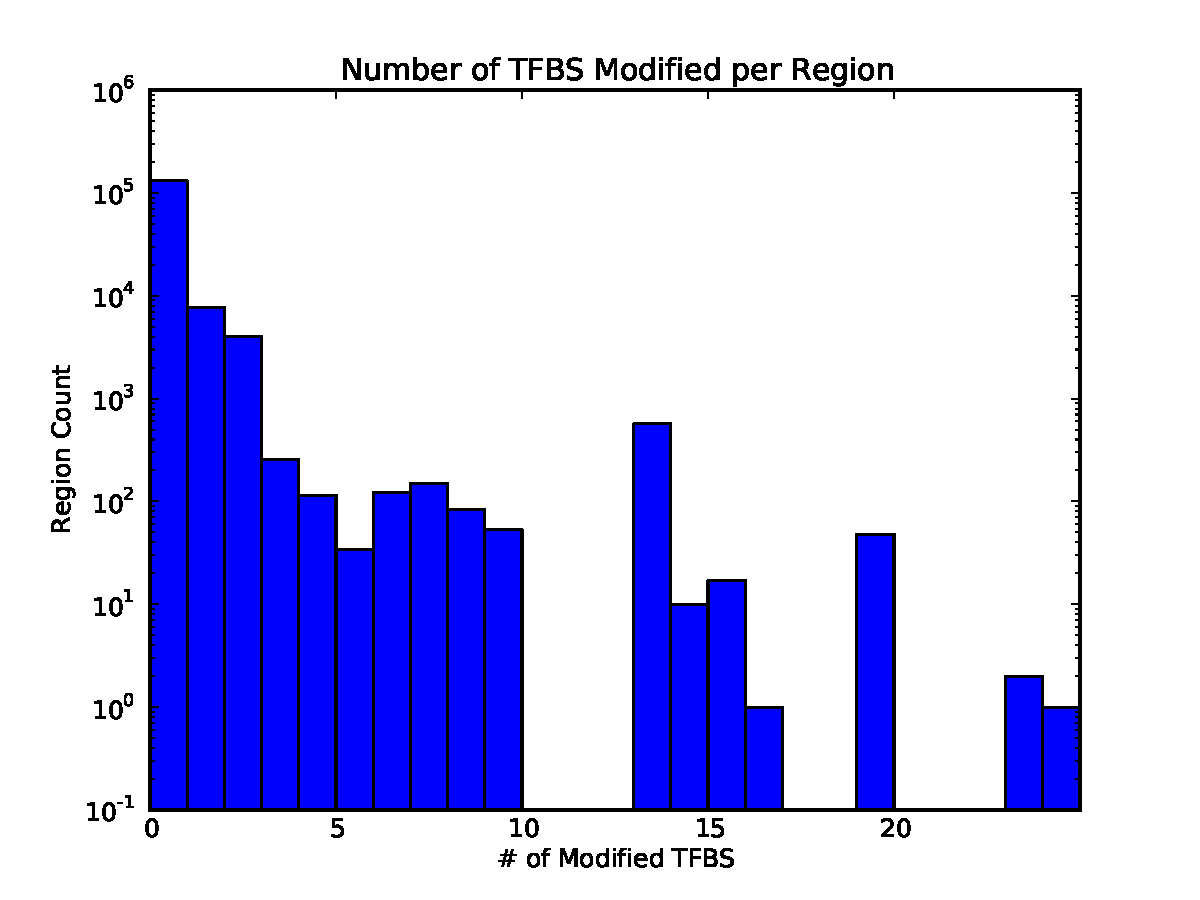
\includegraphics[width=0.25\linewidth]{graphs/mod-sites.pdf}
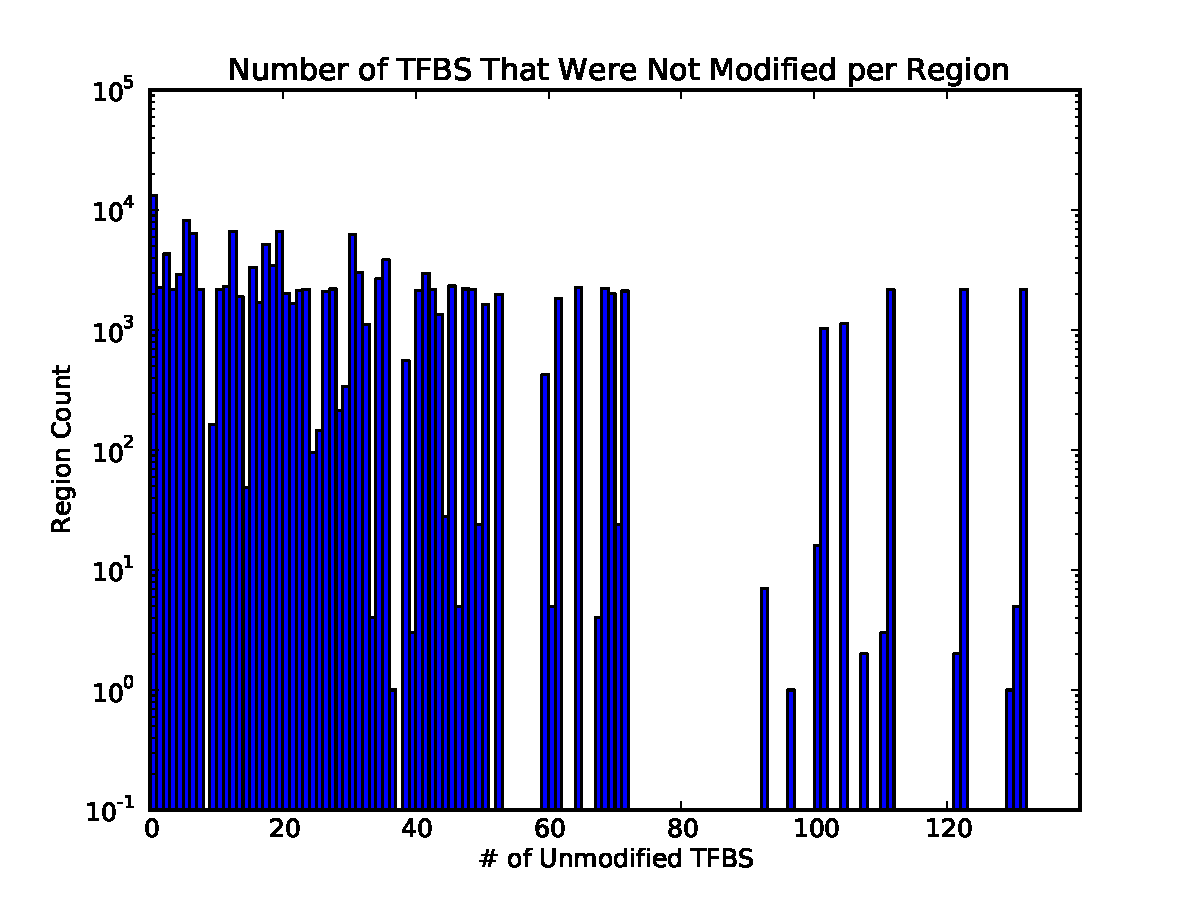
\includegraphics[width=0.25\linewidth]{graphs/unmod-sites.pdf}
\end{center}
\caption{Number of TFBS lost, modified, and unmodified over all regions}
\label{fig:sites}
\end{figure}

Additionally, we would like to do a further review of the modified sites. Specifically,
we would like to look at the degree of modification of these sites, as measured by
the predicted binding affinity of the unmodified site relative to the modified site.

Finally, we looked at changes in spacing between TFBS. These spacing modifications
are caused by INDEL variants. Here, we measure the number of potential TF interactions
that could be gained/lost by a spacing change, under the assumption that two TFs can
interact if they are separated by an interval that is a multiple of 5 bp. This is
shown in Figure~\ref{fig:spacing}. Approximately 89\% of annotated regions did not
see any modified spacing. In the annotated regions that did see modified spacing,
there was no clear distribution of effects. However, it is interesting to note that
the change affects are biased towards \emph{increased} interactions. 

\begin{figure}[h]
\begin{center}
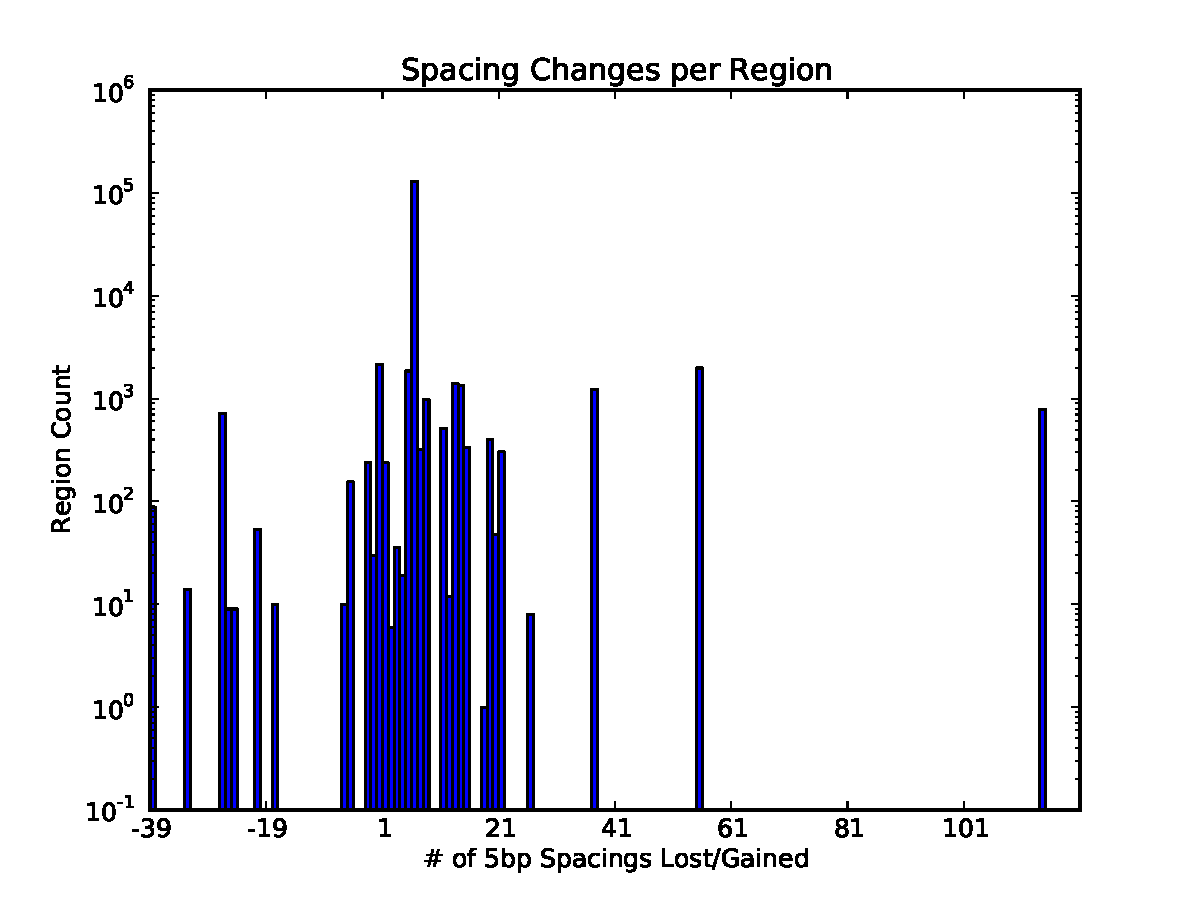
\includegraphics[width=0.25\linewidth]{graphs/spacing.pdf}
\end{center}
\caption{Spacing changes over regions}
\label{fig:spacing}
\end{figure}

There are several additional analyses we would like to incorporate here. Currently,
we do not check to see if two TFs with 5 bp spacing are predicted to interact. This
could be estimated using ENCODE data~\cite{gerstein12}. Additionally, there are odd
gaps/spikes in the spacing changes. We would like to review the data further to see
if there are consistent spacing change motifs.

Additionally, we measured the GC ratio change across regions. Although we did not
compute a change histogram, the average GC ratio change was less than 0.0001\%.
This makes sense, as the GC ratio of 1,500 bp regions will be stable unless we
see very large variants.

\section{Methods}
\label{sec:methods}

\texttt{Fig} is implemented using the \texttt{ADAM} API~\cite{massie13, nothaft15}.
\texttt{ADAM} is a set of data formats and functional operators for processing genomic
datasets on a distributed computing farm, and is built on top of Apache
\texttt{Spark}~\cite{zaharia12, zaharia10}. By building on top of \texttt{ADAM},
\texttt{Fig} is able to rapidly process large datasets. \texttt{Fig} is open source
software under an Apache 2 license and is available from
\url{https://www.github.com/fnothaft/fig}. \texttt{Fig} is decomposed into several steps:

\begin{enumerate}
\item Per region to annotate, extract the reference sequence of the region. We annotate
the reference sequences with TFBS by running a broadcast region join\footnote{A region join
joins tuples from two datasets, where the tuples in each dataset are keyed by the genomic
region that the value in the tuple covers. \emph{Broadcast} implies a specific execution
strategy for the join; specifically, the tuples from the lower cardinality dataset are
broadcast to all of the nodes on the cluster. For more details, see \S5.1 of Nothaft et
al~\cite{nothaft15}.} of the TFBS features against the reference sequences. The binding
affinities of all TFBS are scored using a user-provided position weight matrix~(PWM) per motif.
\item We then compute the ``variant'' regions by loading in the genotypes for all samples,
and running a region join against the reference regions. This effectively labels all
genotypes that are in a region that is to be annotated with the gene ID. From here, we
then group all genotypes together that are from the same sample and that are located in
the region assocated with a single gene ID.
\item Once genotypes are collected by gene and sample, we flatten the variants associated
with these genotypes into haplotypes\footnote{Currently, we only support the processing of
phased genotypes. If the genotypes are unphased, we cannot associate variants to a specific
haplotype. In future work, we hope to add support for unphased genotypes, under some form
of pooled/graph model. This would predict \emph{all possible} modifications. This pooled
model is necessary for processing somatic variant calls, which is a problem we are
interested in.}. The TFBS on these haplotypes are then annotated.
\end{enumerate}

We use a simple algorithm for flattening variants into haplotypes. Starting from
genotypes, we look at the phased genotype states for all genotypes. We do this by
looping over the haplotypes that we are computing. If the genotype call of a genotype
on a specific strand is reference, we discard the variant associated with that
genotype. We the sort the variants associated with a strand by position. We then
run a recursive algorithm that loops over the variants. At each variant, the reference
sequence is replaced by the variant sequence. If the variant is an INDEL, we track the
difference in length between the reference and variant sequences. This difference is
important, as we need it for tracking changes in spacing between TFBS pairs.

We annotate haplotypes using the grammar cards reviewed by Weingarten-Gabbay and
Segal~\cite{weingarten14}. Currently, we support the following annotations:

\begin{itemize}
\item We predict \textbf{changed affinity} by recomputing the TFBS sequence affinity
using the PWM for each TF and the variant and reference sequences. The change in
affinity is expressed as a ratio.
\item We predict the \textbf{loss of a binding site} when the predicted affinity of a
site is reduced to 0 by a variant that modifies the TFBS sequence.
\item We track the \textbf{relative distance} between two TFBS. The TFBS spacing can
be impacted by the presence of INDEL variants. Currently, we track the total number of
TFBS that have spacing that is a multiple of a 5 bp distance, as 5 bp distances lead
to peaks in expression.
\item We compute the GC ratio for the annotated sequences, as a proxy for \textbf{local
sequence context}. This is expressed as a change ratio between the reference and variant
sequence.
\end{itemize}

Eventually, we plan to incorporate these annotations into a GWAS or eQTL pipeline. At
the current moment, we solely use the annotations to calculate a variety of rollups.
Specifically, we calculate the average number of modifications across the dataset,
the average modifications per sample, and the value distributions of each metric
across the whole dataset.

As mentioned above, we built \texttt{Fig} using the \texttt{ADAM} API so that we could
make use of distributed computing to accelerate our analyses. We launched a 32 node
cluster on Amazon's Elastic Compute 2~(EC2) farm to run our analysis of the 1,000 Genomes
dataset. The majority of the runtime~(approximately 1.5 hours out of a two hour job) is
spent executing the region join of genotypes against regions to be annotated. This is
to be expected since the region join discards all genotypes that are outside of the
regions to be annotated, which leads to an approximately 99\% reduction in dataset size.
For efficiency, we have pre-converted the 1,000 Genomes genotype collection from Variant
Call Format~(\texttt{VCF}, \cite{danecek11}) into \texttt{ADAM}'s genotype representation.
This data is stored in the \texttt{eggo} repository~\cite{eggo} and is accessible at
\url{s3://bdg-eggo/1kg/genotypes}. Preconverting to \texttt{ADAM} provides several
advantages: \texttt{ADAM}'s genotype format is 66\% smaller than compressed \texttt{VCF}
and is more efficient to parse, as it is a binary format.

\section{Future Work}
\label{sec:future-work}

In its current state, \texttt{Fig} is capable of annotating regulatory regions with
possible modifications. While this is conceptually useful, \texttt{Fig}'s output is not
meaningfully interpretable. To make \texttt{Fig} a useful tool, we propose extending it
to integrate in with a GWAS/eQTL pipeline. This approach has been proposed previously
by Levo and Segal~\cite{levo14}. This approach could be implemented in multiple forms:

\begin{enumerate}
\item A simplistic annotator could be used to ``filter'' out variants that were predicted
\emph{not} to have an impact on functional regulation. This simplistic annotator would not
necessarily improve the results of a GWAS or eQTL run, but would be useful for eliminating
variants that segregate inside of a LD block that were unlikely to be impactful.
\item A tighter integration of the annotation and eQTL engines could combine the ``grammar
card'' annotations emitted by \texttt{Fig} with the modifications in expression trends
reviewed by Weingarten-Gabbay and Segal~\cite{weingarten14}. While this \emph{could} lead
to better eQTL results, some effects are hard to model (e.g., weak binding affinities).
Additionally, it is not obvious as to how a similar integration would work for annotation
and GWAS.
\end{enumerate}

Additionally, \texttt{Fig} is not a complete annotator. If being used in conjunction with
eQTL/GWAS tools, or in a traditional variant calling and annotation pipeline~(e.g., the
\texttt{GATK} Best Practices Pipeline~\cite{auwera13} or \texttt{HugeSeq}~\cite{lam12}),
it would be useful to annotate coding variants, \emph{a la} \texttt{Annovar}~\cite{wang10}
or \texttt{VEP}~\cite{mclaren10}. Additionally, it would be useful to extend \texttt{Fig}
to annotate more of the functional effect variant cards. Several cards are not annotated
right now (neither nucleosome positioning nor mutual interaction between TFs are predicted,
nor do we predict the \emph{gain} of TFBS due to variants) and would be useful to integrate.

Beyond the fact that \texttt{Fig} is designed for annotating non-coding variants,
\texttt{Fig} differs from traditional variant annotators in that it does not annotate
individual variants, but rather haplotypes. While the approach used by \texttt{Fig}
(specifically, the flattening of variants into haplotypes) works for small datasets,
it is likely that a graph-based approach~(see Novak et al~\cite{novak15}) would be
necessary for annotating larger contiguous regions. While a graph-based approach
doesn't reduce the complexity of annotating a longer contiguous region, a graph-based
approach makes it easier to construct the haplotype that describes the region. For
example, in a string-based haplotype annotator, all variants on a single phased
branch of a chromosome would need to be collected together and integrated serially
into the haplotype. In a graph-based haplotype annotator, individual variants modify
a limited portion of the overall graph.

As mentioned earlier, a future aim for this project is to add support for somatic
callsets under a pooled annotation model. We originally were targeting The Cancer
Genome Atlas~\cite{weinstein13}, but refocused on the 1,000 Genomes project due to
issues surrounding data access and quality. Long term, our interest is in using the
annotation of regulatory variants to look at diseases such as Acute Myeloid Leukemia~(AML),
which are known to have very few coding variants~\cite{cancer13}.

\section{Conclusion}
\label{sec:conclusion}

In this paper, we presented \texttt{Fig}, a haplotype-based tool for annotating
variants that overlap with regulatory regions. \texttt{Fig} is built on top of the
\texttt{ADAM} API, and is designed for processing very large datasets. We have
demonstrated \texttt{Fig} on the genotype calls from the 1,000 Genomes dataset,
and have plotted future enhancements for the \texttt{Fig} project, which include
integration with GWAS/eQTL tools.

\bibliographystyle{abbrv}
\bibliography{fig}

\end{document}
